
\setchapterimage[6cm]{cabecera}
\setchapterpreamble[u]{\margintoc}
%%%%%%%%%%%%%%%%%%%%%%%%%%%%%%%%%%%%%%%%%%%%%%%%%%%%%%%%%%%%%

\chapter{Protocolos de la capa de Transporte }
\label{ch:Potocolos capa de Transporte}
\index{potocolos capa de transporte}

Este capítulo trata acerca de las interfaces de los programas de aplicación (API), en particular de las interfaces entre los programas de aplicación y el protocolo TCP/IP.  
En arquitecturas cliente-servidor, cuando se hace una solicitud, por ejemplo obtener una imagen, image.png de la página web example.com ,  los pasos que se siguen, a grandes rasgos, son los siguientes:

\begin{enumerate}
	\item Obtener una dirección ip para example.com (descrito en la sección acerca del DNS, ver \ref{cap:DNS}).
	\item Abrir un \textit{socket} a una dirección ip en un puerto determinado
	\item Abrir una conexión TCP a una dirección ip en un puerto determinado
	\item Hacer la solicitud HTTP GET, de la image.png
	\item Obtener la imagen solicitada, image.png
	\item Cerrar la conexión.
\end{enumerate}
En lo que sigue, se detalla el concepto de  \textit{socket}.

\section{Socket} \index{socket}

La abstracción de la interfaz \textit{socket} es el socket \sidecite{Comer2014}, \sidecite{Peterson2021}. Un socket es como el punto donde un proceso de aplicación local se conecta a la red. La interfaz define las operaciones de creación del socket, adjuntar el socket a la red, enviar/recibir mensajes a través del socket y cerrar el socket.  como se ilustra en la figura \ref{fig:socket}.
 
Para que un proceso reciba mensajes, su socket debe estar vinculado a un puerto local y a una de las direcciones de Internet en la computadora  que se ejecuta. 
Los mensajes enviados a una dirección de Internet y número de puerto en particular solo pueden recibir un proceso cuyo socket está asociado con esa dirección de Internet y número de puerto.

Los \gls{procesos} pueden usar el mismo socket para enviar y recibir mensajes.   
Cualquier proceso puede hacer uso de múltiples puertos para recibir mensajes, pero un proceso no puede compartir puertos con otros procesos en la misma computadora. 
Cada socket esta asociado con un protocolo particular, ya sea \textit{UDP} o \textit{TCP}.


\begin{figure}%
	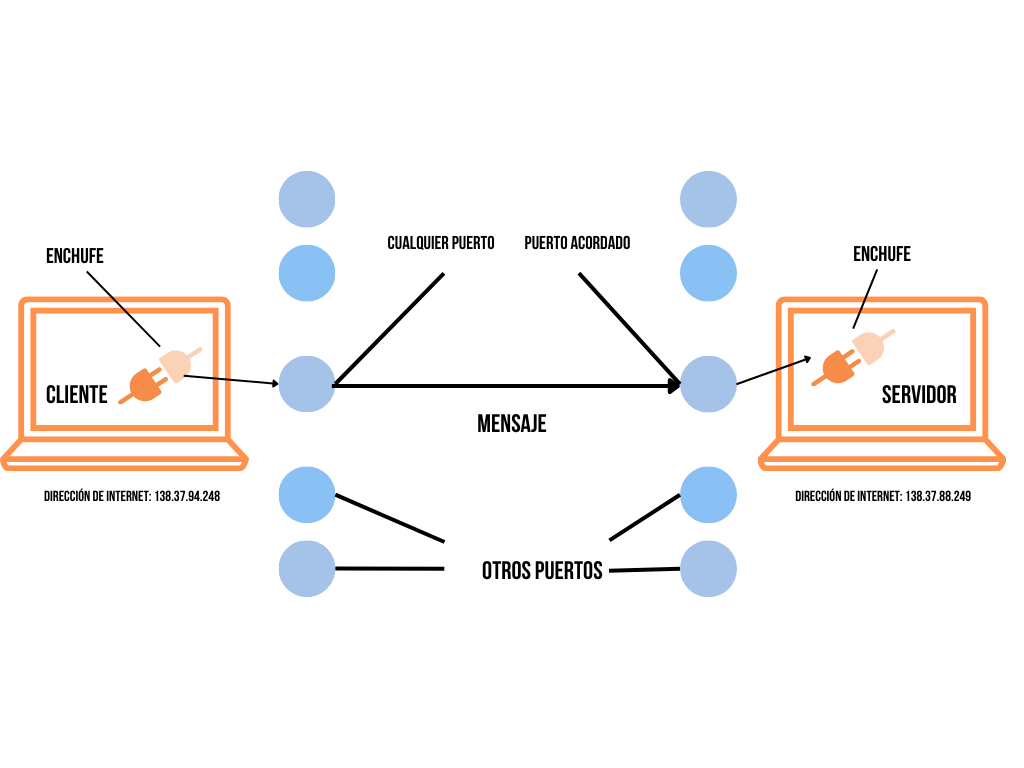
\includegraphics[width=0.8\textwidth]{4/15.png}
	\caption{Socket.}
	\label{fig:socket}
\end{figure}

Veamos como se implementan los socket en los protocolos de la capa de transporte, UDP y TCP.

%------------------------------------------------------	
\section{UDP}
%------------------------------------------------------	
\textit{UDP},\textit{User Datagram Protocol}, es un protocolo de nivel de transporte basado en el intercambio de datagramas. Permite el envío de datagramas a través de la red sin que se haya establecido previamente una conexión, ya que el propio datagrama incorpora suficiente información de direccionamiento en su cabecera. No tiene confirmación de recepción del mensaje ni control de flujo de transmisión del mensaje, por lo que los paquetes pueden adelantarse unos a otros; y tampoco se sabe si ha llegado correctamente, ya que no hay confirmación de entrega o recepción .
 \index{UDP}

Un datagrama enviado por UDP se transmite desde un proceso de envío a un proceso de recepción sin reconocimiento ni reintentos. Si ocurre una falla, el mensaje puede que no llegue.   Para enviar o recibir mensajes, un proceso primero debe crear un socket vinculado a una dirección de Internet del \textit{host} local y un puerto local. El  servidor enlazará su socket a su puerto: y se da a conocer a los clientes para que puedan enviarle mensajes. 
\index{datagram}  \index{User Datagram Protocol}

	\begin{kaobox}[frametitle=Datagrama]
		En la capa de transporte, la unidad de transferencia básica en las llamadas de internet son los datagramas de internet, llamados también datagramas IP o \gls{datagrama}.
		 La capa de transporte es responsable de brindar servicios a la capa de aplicación: obtener un mensaje de un programa de aplicación que se ejecuta en el host de origen; lo encapsula en un paquete de capa de transporte (llamado datagrama de usuario);  y entregarlo al programa de aplicación correspondiente en el host de destino.
		 Un datagram esta compuesto de dos partes: encabezado y cuerpo, en la figura \ref{fig:datagram} se ilustra la estructura.
		 
	  	Revisar m\'as de \textit{UDP} en documento de \textit{IBM}:  \href{https://www.ibm.com/docs/es/aix/7.1?topic=protocols-user-datagram-protocol}{UDP}
		
\end{kaobox}  

	\begin{figure}
		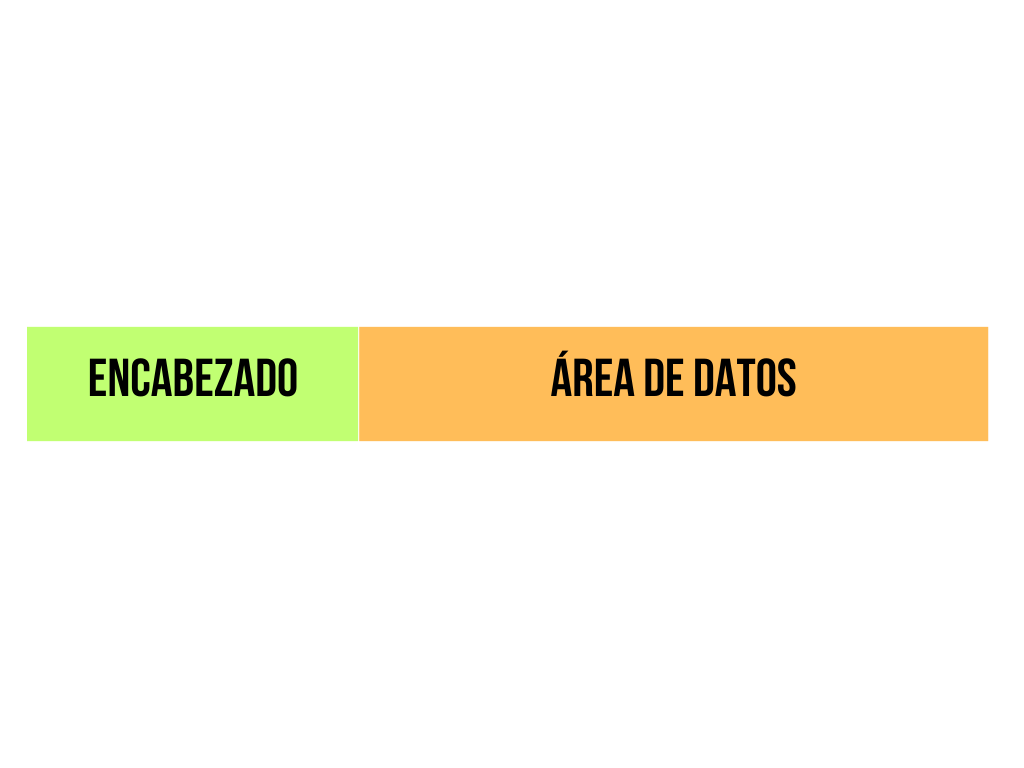
\includegraphics[width=0.8\textwidth]{4/18.png}
		\caption{Estructura del Datagrama}
		\label{fig:datagram}
	\end{figure} 


Los siguientes son algunas caracteristicas relacionada  con la comunicación de datagramas \sidecite{Forouzan2021}:
\begin{description}
	\item [Tamaño del mensaje:] la longitud total de un datagrama esta medido en octetos.
	\index{tama\~no mensaje en UDP}
	\begin{itemize}
		\item Longitud del encabezado (HLEN). El campo de longitud del encabezado de 4 bits (HLEN) define la longitud total del encabezado del datagrama en palabras de 4 bytes. El datagrama IPv4 tiene un encabezado de longitud variable. Cuando un dispositivo recibe un datagrama, necesita saber cuándo se detiene el encabezado y comienzan los datos, que están encapsulados en el paquete. Para que el valor de la longitud del encabezado (número de bytes) se ajuste a una longitud de encabezado de 4 bits, la longitud total del encabezado se calcula como palabras de 4 bytes. La longitud total se divide por 4 y el valor se inserta en el campo.
		\item Longitud total. Es un campo de 16 bits  (encabezado más datos) del datagrama IP en bytes. Un número de 16 bits puede definir una longitud total de hasta 65.535. Sin embargo, el tamaño del datagrama es normalmente mucho menor que esto. Para encontrar la longitud de los datos de un datagrama, reste la longitud del encabezado de la longitud total. La longitud del encabezado se puede encontrar multiplicando el valor en el campo HLEN por 4:
		
		\begin{kaobox}
		\small{\textbf{Longitud de datos = longitud total - (HLEN) x 4}}
		\end{kaobox}   
		
	\end{itemize}
	
	\item[Bloqueos:]  La implementación de sockets con datagramas  normalmente proporcionan envíos sin bloqueo y recepciones con bloqueo (una recepción sin bloqueo es una opción en algunos implementaciones): 
	\begin{itemize}
		\item La operación de envío termina cuando ha entregado el mensaje a los protocolos UDP e IP subyacentes, que son responsables de transmitirlo al host de destino. 
		\item A su llegada al destino, el mensaje se coloca en una cola asociada al puerto de destino que esta relacionado con el socket. 
		\item El mensaje puede ser recogido de la cola por un invocación pendiente o futura a ese socket. 
		\item Los mensajes se descartan en 	el destino si no hay  procesos  con un socket vinculado al puerto de destino.
	\end{itemize} \index{bloqueo en UDP}
	
	\item[Tiempos de espera:]     La recepción con bloqueo   es adecuada cuando un servidor está esperando recibir solicitudes de sus clientes. Pero en algunos programas, no es apropiado que en procesos que han invocado una operación de recepción con espera, lo haga indefinidamente. Puede suceder fallas en el proceso de envío  o el mensaje esperado puede haberse	perdido. Para ello, se pueden establecer tiempos de espera en los sockets. 
	\index{tiempo de espera en UDP}
	
	\item[Recibir de cualquiera:] el método de recepción no especifica un origen para los mensajes. En cambio, una invocación del m\'etodo de  recepci\'on obtiene un mensaje dirigido a su socket desde cualquier	origen. El método de recepción devuelve la dirección de Internet y el puerto local del remitente, 	permitiendo al destinatario comprobar de dónde procede el mensaje. Es posible conectar un \textit{socket} de datagrama a un puerto remoto particular y una dirección de Internet, para  que el \textit{socket} pueda enviar mensajes y recibir mensajes de esa direcci\'on. 
	\index{recepci\'on de mensajes en UDP}
\end{description}
 

%------------------------------------------------------	
\subsection{Uso de UDP }  
%------------------------------------------------------	 
\index{uso de UDP}
Voz sobre IP y DNS:    Es una opción popular  porque no causa sobrecarga (\textit{overhead}) en la red
 

%------------------------------------------------------	
\section{TCP}
%------------------------------------------------------	
A diferencia del protocolo \textit{UDP}, \textit{TCP} es un protocolo que ofrece un servicio de flujos de bytes, fiable y orientado a la conexión. Dicho servicio ha demostrado ser útil para una amplia variedad de aplicaciones porque libera a la aplicación de tener que preocuparse sobre datos perdidos o reordenados, \sidecite{Comer2014}. 

El protocolo de control de transmisión (\textit{Transmission Control Protocol} o TCP) es uno de los protocolos fundamentales en Internet. Los programas  pueden usar TCP para crear “conexiones” entre sí a través de las cuales puede enviarse un flujo de datos.
\index{TCP}

TCP da soporte a muchas de las aplicaciones de Internet (navegadores, intercambio de ficheros, clientes FTP, etc.) y protocolos de aplicación, \sidecite{Peterson2021}, \sidecite{Forouzan2021} :
\begin{description} \index{protocolos}
	\item[HTTP]   \gls{HTTP},  protocolo de transferencia de hipertexto,   se utiliza para la comunicación entre los navegadores web y servidores web.
	
	\item[FTP]  el Protocolo de transferencia de archivos permite que los directorios en una computadora remota naveguen y transferir archivos para ir de una computadora a otra a través de una conexión.
	
	\item[Telnet]  Telnet proporciona acceso mediante una sesión de terminal a una computadora remota.
	
	\item [SMTP] el Protocolo  de transferencia de correo se utiliza para enviar correo entre computadoras.
\end{description}

En la figura \ref{fig:TCP-suite}  se muestra la posición de IP y de los protocolos de la capa de red, en conjunto con la grupo de protocolos  de TCP/IP ya descritos (se han omitido los protocolos por debajo de la capa de Red).


\begin{figure}
    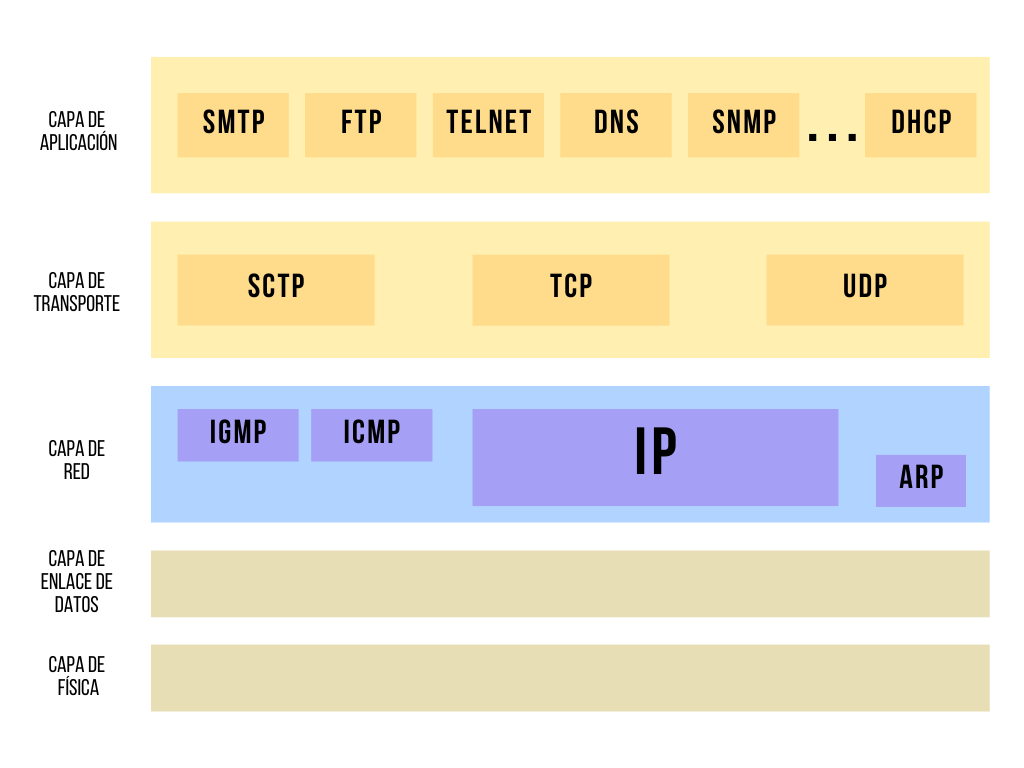
\includegraphics[width=0.9\textwidth]{4/19.png}
    \caption{Protocolos TCP/IP}
    \label{fig:TCP-suite}
\end{figure}

Las  características de TCP son las siguientes:
\begin{description}    \index{caracter\'isticas de TCP}
	\item[Tamaños de mensaje:]   la aplicación puede elegir cuántos datos escribe o lee en un segmento. Puede tratar conjuntos de datos muy pequeños o muy grandes. La implementación de una secuencia o segmento TCP decide cuántos datos recopilar antes de  transmitirlo como uno o más paquetes IP. A su llegada, los datos se entregan a la aplicación según lo solicitado.   \index{tama\~no mensaje en TCP}
	
	\item [Mensajes perdidos:] el protocolo TCP utiliza un esquema de reconocimiento del mensaje. Por ejemplo,  el extremo emisor mantiene un registro de cada paquete IP enviado y el extremo receptor reconoce todas las solicitudes recibidas y envía un acuse de recibo. Si el remitente  no recibe un acuse de recibo de un mensaje dentro de un tiempo de espera, entonces  retransmite el mensaje.  \index{mensajes perdidos en TCP}
	
	\item [Control de flujo:] TCP intenta igualar las velocidades de los procesos de lectura y escritura en un segmento. Si el escritor es demasiado rápido para el lector, entonces es 	bloqueado hasta que el lector haya consumido suficientes segmentos de datos. \index{control de flujo en TCP}
	
	\item [Duplicación y ordenamiento de mensajes:] los identificadores de mensajes están asociados con cada paquete IP, que permite al destinatario detectar y rechazar duplicados, o reordenar los	mensajes que no llegan en el orden del remitente. \index{orden de mensajes en TCP}
	
	\item[Destinos de mensajes:]   un par de procesos de comunicación establecen una conexión antes de que puedan comunicarse a través de una secuencia. Una vez que se establece una conexión, 	Los procesos  leen y escriben los \textit{stream} de datos sin necesidad de utilizar 	direcciones  de Internet o puertos. Establecer una conexión implica una solicitud de conexión del cliente al servidor seguido de una solicitud de aceptación del servidor al cliente antes que cualquier comunicación puede tener lugar.  \index{destino de mensajes en TCP}	
\end{description}

\subsection{Mensajes de TCP}

TCP es un protocolo orientado a bytes, significa que el remitente escribe bytes en una conexión TCP y el receptor lee bytes de la conexión TCP, \sidecite{Peterson2021}, \sidecite{Coulouris2011}. 
TCP no transmite bytes individuales a través de Internet.  En su lugar, TCP en el host origen almacena suficientes bytes del proceso de envío para llenar un paquete de tamaño razonable y luego envía este paquete a su par en el host destino. TCP en el host destino  vacía el contenido del paquete en un búfer de recepción, y el proceso de recepción lee de este búfer en su tiempo libre. 

En la figura \ref{fig:TCP-segmento}, muestra este intercambio de  datos  en una  dirección; aunque,  una única conexión TCP admite flujos de bytes que fluyen en ambas direcciones.

Los paquetes intercambiados entre pares TCP en la Figura \ref{fig:TCP-segmento} son segmentos, ya que cada uno lleva una parte del flujo de bytes.


\begin{figure}
	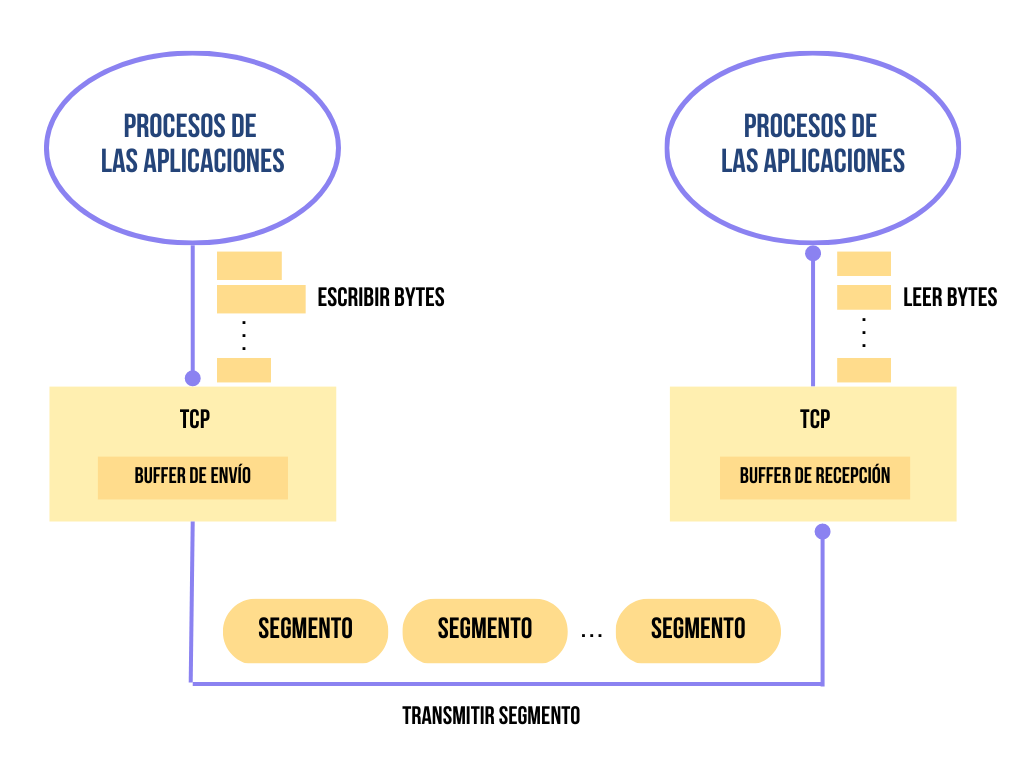
\includegraphics[width=0.9\textwidth]{4/20.png}
	\caption{Intercambio de mensajes en TCP}
	\label{fig:TCP-segmento}
\end{figure}

 
La estructura del segmento se muestra  en la Figura \ref{fig:TCP-seg-estruc}. 
\begin{itemize}
	\item  \textbf{SrcPort} y \textbf{DstPort} identifican el origen y el destino de los puertos, al igual que en UDP. Estos campos, más la dirección de lafuente y las IP de destino, identifican cada conexión TCP. 
	\item El campo  \textbf{número de secuencia} contiene el número de secuencia para el primer byte de datos 	transportado en ese segmento.
	\item  Los campos \textbf{Reconocimiento} y \textbf{AdvertisedWindow} llevan información sobre el flujo de datos que van en la dirección contraria.
	\item El campo \textbf{banderas}  se utiliza para transmitir información de control entre los puntos de conexión TCP.  Los indicadores posibles incluyen SYN, FIN, RESET, PUSH, URG y
	ACK. Por ejemplo, las banderas \textbf{SYN} y \textbf{FIN} se utilizan al establecer y terminar una conexión TCP, respectivamente
	\item  El campo \textbf{HdrLen} da la longitud del encabezado en palabras de 32 bits. Este campo  se conoce como campo de desplazamiento, ya que mide el desplazamiento desde el inicio del paquete hasta el comienzo de los datos.
	\item El campo \textbf{Checksum} se usa  de la misma manera que para UDP: se calcula sobre el encabezado TCP, los datos TCP y el pseudoencabezado, que se compone de la dirección de origen, la dirección de destino y la longitud 	campos del encabezado IP. La suma de comprobación es necesaria para TCP tanto en IPv4
	e IPv6. 
\end{itemize}

\begin{figure}
	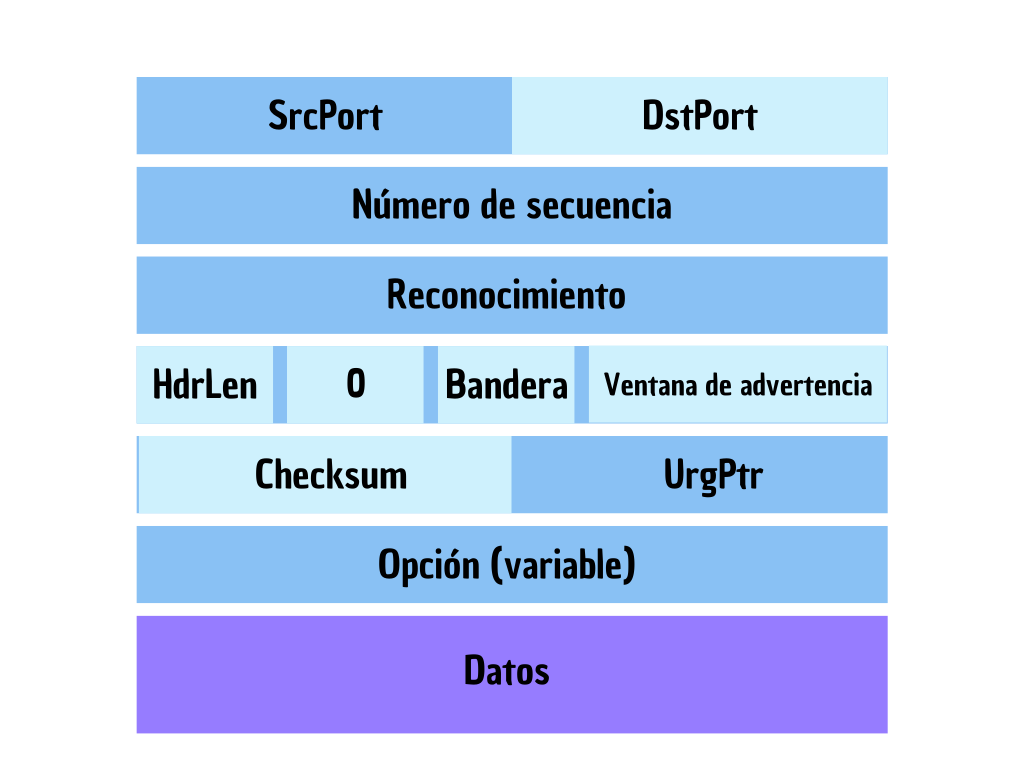
\includegraphics[width=0.9\textwidth]{4/21.png}
	\caption{Estructura de mensajes en TCP}
	\label{fig:TCP-seg-estruc}
\end{figure}
 


%------------------------------------------------------	
\section{Multidifusi\'on }
%------------------------------------------------------	 

Una operación de multidifusión (\textit{multicast}) es  una operación que envía un   mensaje de un proceso a cada uno de los miembros de un grupo de procesos, de manera que la membresía  del grupo es transparente para el remitente. Hay un abanico de posibilidades en el   comportamiento de una multidifusión. El protocolo de multidifusión más simple no ofrece garantías sobre  envío de mensajes o mensajes perdidos.
\index{multidifusi\'on}

Los mensajes de multidifusión proporcionan una infraestructura  para construir sistemas distribuidos  con las siguientes características:
\begin{enumerate}
	\item  Tolerancia a fallas basada en servicios replicados: un servicio replicado consta de un  grupo de servidores para suplir un servicio en particular. Las solicitudes de los clientes se envían por multidifusión a todos los miembros del grupo de servidores,  cada uno de los cuales realiza una operación idéntica. Cuando algunos de los miembros
	falla, los clientes aún pueden ser atendidos.  \index{tolerancia a fallas}
	
	\item Descubrimiento de servicios en redes espontáneas: En el \gls{descubrimiento de servicios}, se usan los mensajes de multidifusión por servidores y clientes para localizar los servicios de  disponibles con el fin de  registrar sus interfaces o buscar las interfaces de otros servicios en el  Sistema distribuido.  \index{descubrimiento de servicios}
	
	\item  Mejor rendimiento a través de datos replicados: los datos se replican para aumentar el  rendimiento de un servicio: en algunos casos, las réplicas de los datos se colocan en los computadores de usuarios. Cada vez que cambian los datos, el nuevo valor se envía por multidifusión a los procesos que gestionan las réplicas.  \index{datos replicados}
	
	\item Propagación de notificaciones de eventos: la multidifusión a un grupo se puede utilizar para notificar  a procesos cuando algo sucede. Por ejemplo, en Facebook, cuando alguien  cambia su estado, todos sus amigos reciben notificaciones.   \index{notificaciones de eventos}
	
\end{enumerate}
%%%%%%%%%%%%%%%%%%%%%%%%%%%%%%%%%%%%%%%%%%%%%%%%%%%%%%%%
\subsection{La multidifusión IP} La multidifusión IP  se basa en el Protocolo de Internet (IP).  Multidifusión IP permite al remitente transmitir un solo paquete IP a un conjunto de computadoras que forman un grupo de multidifusión. 
La multidifusión IP tiene las siguientes características:
\begin{description}
	\item[Dirección de Grupos.] Cada grupo de multidifusión es una direción única de la clase D. Unas pocas direcciones son asignadas por la autoridad única de internet, otras direcciones son de uso privado. 

	\item[Número de Grupos.] IP proporciona direcciones hasta para $2^{28}$ grupos de multidifusión.
	\item[Membresía dinámica a grupos.] Un host puede unirse o abandonar un grupo de IP multidifusión cuando lo requiera.
	\item[Uso del hardware.] Si el hardware de la red subyacente soporta IP multidifusión, entonces IP usa el hardware de multidifusión para enviar los mensajes IP multidifusión. En caso contrario, usa difusión(cast) o transmisión (broadcast)
	\item[Reenvio en Redes.] Debido a que miembros de grupos de multidifusión IP son adjuntos a varias redes físicas, se require el uso de enrutadores con la capacidad de multidifusión para el reenvío de multidifusión IP.
	\item[Semántica de la distribución] Multidifusión IP usa la \gls{semantica  mejor-esfuerzo}para la distribución de mensajes: significa que un datagrama multidifusión puede perderse, retrasarse, duplicarse, o distribuirse fuera de orden  
	\item[Membresía y transmisión.] Un host arbitrario puede enviar datagramas al grupo de multidifusión. La membresía al grupo solo se usa para determinar si el datagrama recibido por el host puede ser enviado al grupo.
\end{description}



En el nivel de programación de aplicaciones, la multidifusión IP solo está disponible a través de UDP. 
Un  programa de aplicación realiza multidifusión enviando datagramas UDP con multidifusión  direcciones y números de puerto ordinarios. Puede unirse a un grupo de multidifusión haciendo que su socket se una  al grupo, lo que le permite recibir mensajes al grupo. A nivel de IP, una computadora pertenece a un grupo de multidifusión cuando uno o más de sus procesos tiene sockets que pertenecen  a ese grupo. Cuando llega un mensaje de multidifusión a una computadora, las copias se reenvían a  todos los sockets locales que se han unido a la dirección de multidifusión especificada y están vinculados a
el número de puerto especificado. 
%%%%%%%%%%%%%%%%%%%%%%%%%%%%%%%%%%%%%%%%%



%%%%%%%%%%%%%%%%%%%%%%%%%%%%%%%%%%%%%%%%%%%%%%%%%%%%%%%%%%%%%%


\section{Caso de Estudio: ?`Como funciona un aplicación de Chat?}
\index{caso de estudio!?`como funciona un aplicación de chat?}

Este ejemplo se muestra como se usan los protocolos de comunicación en una aplicación Chat.
Un chat es un tipo de comunicación en tiempo real que se realiza entre varios usuarios cuyas computadoras están conectadas a una red, generalmente Internet; los usuarios escriben mensajes en su teclado, y el texto aparece automáticamente y al instante en el monitor de todos los participantes.
Ejemplo de aplicaciones chat son Whatsapp, Google Chat, Skype, entre otras.

\begin{figure}
	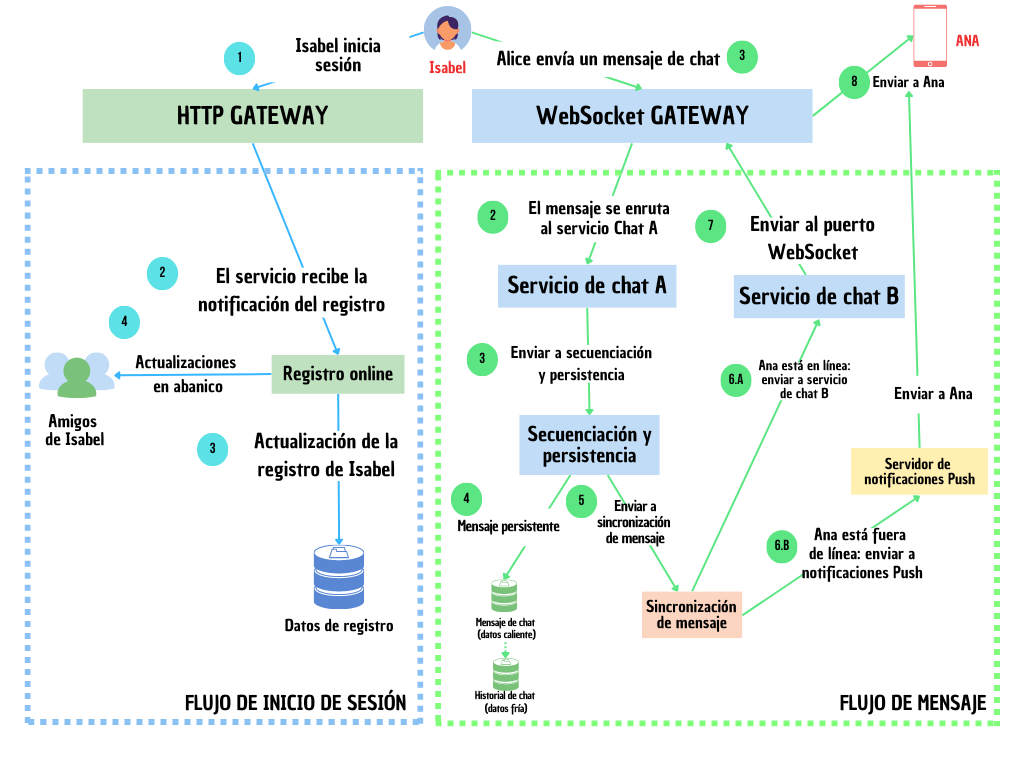
\includegraphics[width=0.9\textwidth]{4/22.png}
	\caption{Chat. Adaptado de {\cite{Xu2022}}}
	\label{fig:chat}
\end{figure}

A continuación, se describe el funcionamiento, de una aplicación chat, de acuerdo a la  figura \ref{fig:chat}, \sidecite{Xu2022}.

\paragraph{Flujo de inicio de sesión de usuario}

\begin{itemize}
	\item 1: Isabel inicia sesión en la aplicación de chat y establece una conexión de socket web con el lado del servidor.
	\item 2-4: El servicio  recibe  la notificación del registro de Isabel, actualiza su registro y notifica a los amigos de Isabel sobre su presencia.
\end{itemize}

\paragraph{Flujo de mensajería}
\begin{itemize}
	\item  5: El mensaje de chat se envía a la cola de sincronización de mensajes para sincronizar con el servicio de chat de Ana.
	\item 6: antes de reenviar el mensaje, el servicio de sincronización de mensajes verifica la presencia de Ana:
	 	\begin{enumerate}
	 		\item   Si Ana está en línea, el mensaje de chat se envía al servicio de chat B.
	 		\item Si Ana está desconectada, el mensaje se envía al servidor push y se envía al dispositivo de Ana.
	 	\end{enumerate}	
	\item  si Ana está en línea, el mensaje de chat se envía a Ana a través del socket web.
\end{itemize}
 






